\autsection{Technical Plan}{Nelián Colón, Samuel Rodríguez and Daniel Santiago}

\subsection{Web Application}

Panda Code Reviews is a fully hosted web application. The web application
includes many parts, the main of these are the front end and the back end. The
front end is what the user sees and interacts with directly. It is very
important to design the front end with ease of use in mind, and almost equally
important is designing the interface with a clean and modern look. The back end
is the underlying software that manages the communication between the front end
interface and the database, repository manager and testing framework. The front
end and the back end are connected in various parts, so this must be properly
designed for ensuring compatibility and hassle-free communication. For example,
data passing between the database and the front end through the back end must
be concise, so a standard object model should be used. It is discussed in the
following sections the usage of JSON objects for this purporse. Additionally,
the URL end points of the application must be specified for compatibility
between the front end and the back end.

\subsection{Front end}

As mentioned earlier, it is very important to design the front end interface
with ease of use in mind, and it is also very important to design the interface
with a clean and modern look. The Model-View-Controller (MVC) pattern is being
followed for developing the front end. The idea of the MVC pattern is to have an
good organization in the code between managing the application's data (model),
the application's logic (controller), and the application's presentation (view).
The view gets data from the model to display to the user. When a user interacts
with the application, the controller changes data in the model, and the data
gets passed from the model to the view so that it is displayed to the user. In
the case of Panda Code Reviews, the view of the application is the Document
Object Model (DOM) of the web pages. The controller of the application is
JavaScript code that uses AngularJS, and the model data is all stored in JSON
objects.

One of the most difficult tasks in developing the front end of the application
is ensuring good compatibility between the model, the view and the controller.
AngularJS makes this compatibility easier by providing a type of templating
engine in the client side. It allows for automatic refreshing of data. For
example, if the controller of the application changes the model data, AngularJS
automatically refreshes the view so that it gets displayed to the user. And if
the view is changed by the user, AngularJS can automatically update the model.

\subsubsection{View}

The view is being handled by HTML and CSS. Panda Code Reviews uses Bootstrap, an
open source front end framework for faster and easier development of the front
end's view. It provides many CSS classes for easily templating the web pages. It
is also highly customizable, and provides a JavaScript plugin interface for
enabling animations and other features like component pinning. These plugins
might be activated by the controller or by other means such as after a page
loads.

\subsubsection{Controller}

The controller of the front end is being developed in JavaScript. JavaScript is
implemented by all major browsers and provides a very comprehensive standard
library for manipulating elements of the DOM and registering event listeners.
JQuery, a comprehensive JavaScript library, is being used for simplifying and
reusing many routines. Also, AngularJS is being used for simplifying
communication between the model, the view and the controller. More will be
discussed about AngularJS in the next section.

\subsubsection{Model and Communication}

The model of the application is embedded in the controller and specified in the
database, which the front end has no direct access to. Instead, the front end
will communicate with the back end through a REST API, and the back end will
answer the front end's query with JSON objects. AngularJS, an open source
templating framework, will be used for simplifying the communications between
the front end's controller and model. AngularJS will also be used for
communicating with the back end through its REST API. When the user interacts
with the front end's view, AngularJS responds by changing the model in the front
end, which will then call the necessary controller functions that will
communicate with the back end through its REST API. The back end will respond to
the controller's query with JSON objects, and AngularJS will manage the change
of data between the controller, the model and the view. AngularJS is also highly
modifiable, so some functionality is overriden so that it better suits Panda
Code Review's functionalities.

\subsubsection{Views}
% Parenthesis means that no mock exists yet.
Index

Login
(Sign Up)

Account Home

Course (Falta professor, create course | edit mode)

Assignment (falta edit mode, create assignment)
	Info
	Submissions
	Test Cases
	Repositories (Gitlab)

(Admin panel)
	(Schools)
	(Server status)

(Account Settings (Profile))
(Professor's side of grading)


\subsection{Back end}

The back end is the underlying server side software that manages the
communication and flow between the front end and the database server, the
repository manager, and the testing framework. The front end sends requests for
data to the back end using its REST API. The back end then proceeds with
establishing a connection to the MongoDB database server and then passing the
query's result to the front end. The database server returns query results with
JSON objects, and the back end does not have to translate this information in
any way, since the front end also uses JSON objects as discussed in the earlier
sections. The back end is also responsible of instantiating the sand boxes where
the submitted code and test cases will run. This is also invoked by orders of
the users when they interact with the front end of Panda Code Reviews.

% usar palabra fancy: serialization and deseriaization. Si fuera SQL, habria
% que hacer todas esas cosas.

\subsubsection{Node.js}

% a~nadir  footnotes explicando.

The back end service is being build in JavaScript using Node.js. Node.js is a
platform built on Google Chrome's Open Source V8 JavaScript runtime engine for
easily building fast and scalable network and server-side applications. It uses
JavaScript as its scripting language and achieves high throughput via an event
driven, non-blocking I/O model on a single-threaded event loop. It also contains
a built-in HTTP server library, which allows for easy deployment of a web server
without the need of external HTTP servers like Apache, Lighttpd or Nginx.
Node.js poses additonal ease of use when it comes to interacting with MongoDB,
since it uses JSON-style documents as well. This means that no additional
library or wrapper is needed to communicate with the database.

\subsubsection{GitLab}

GitLab is open source software to help developers collaborate on code. It can be
used to create projects and repositories and manage access.

\subsubsection{Endpoints}

\subsubsection{Codeworkers}

\subsection{Database}

The database is used for storing all required information about the system and
its users.

\subsubsection{MongoDB}

MongoDB is a cross-platform document-oriented database system. It is classified
as a NoSQL database which provides a mechanism for storage retrieval that is not
as constrained as relational databases like MySQL or PostgreSQL. MongoDB
features JSON-style (JavaScript Object Notation) documents with dynamic schemas,
which allows simpler and quicker development. A dynamic schema approach enables
flexibility for quickly changing applications, and the JSON style documents
provide a unified language for passing database objects between the Node.js
backend and the front end, both written entirely in Javascript. MongoDB is the
leading NoSQL DBMS, it is more stable than its closest competitor Redis.

\subsubsection{Entity-Relationship Diagram}

The collections have been defined following two different approaches: the
standard ER diagram that defines entities and the relationships with each other
and a JSON-like diagram that better models MongoDB's Documents and Collections.
Overall, we created structures for users (Administrators, Professors, Students
and TAs), courses, assignments and submissions.


\subsection{Deployment}

Continuous development has been set up in the deployment server colocated at
Amazon's EC2 infrastructure. This enables an always working version hosted in
the cloud which gets automatically deployed whenever a developer pushes code to
the master branch in Git. When the latest version is pushed, the Node Package
Manager (NPM) runs code tests to make sure that the latest push is healthy. If
it passes the tests, the server is shut down, any new dependencies are installed
with NPM, and the server is restarted with the new changes in effect. This all
happens automatically.

% This is the overview of the front end and back end architecture.
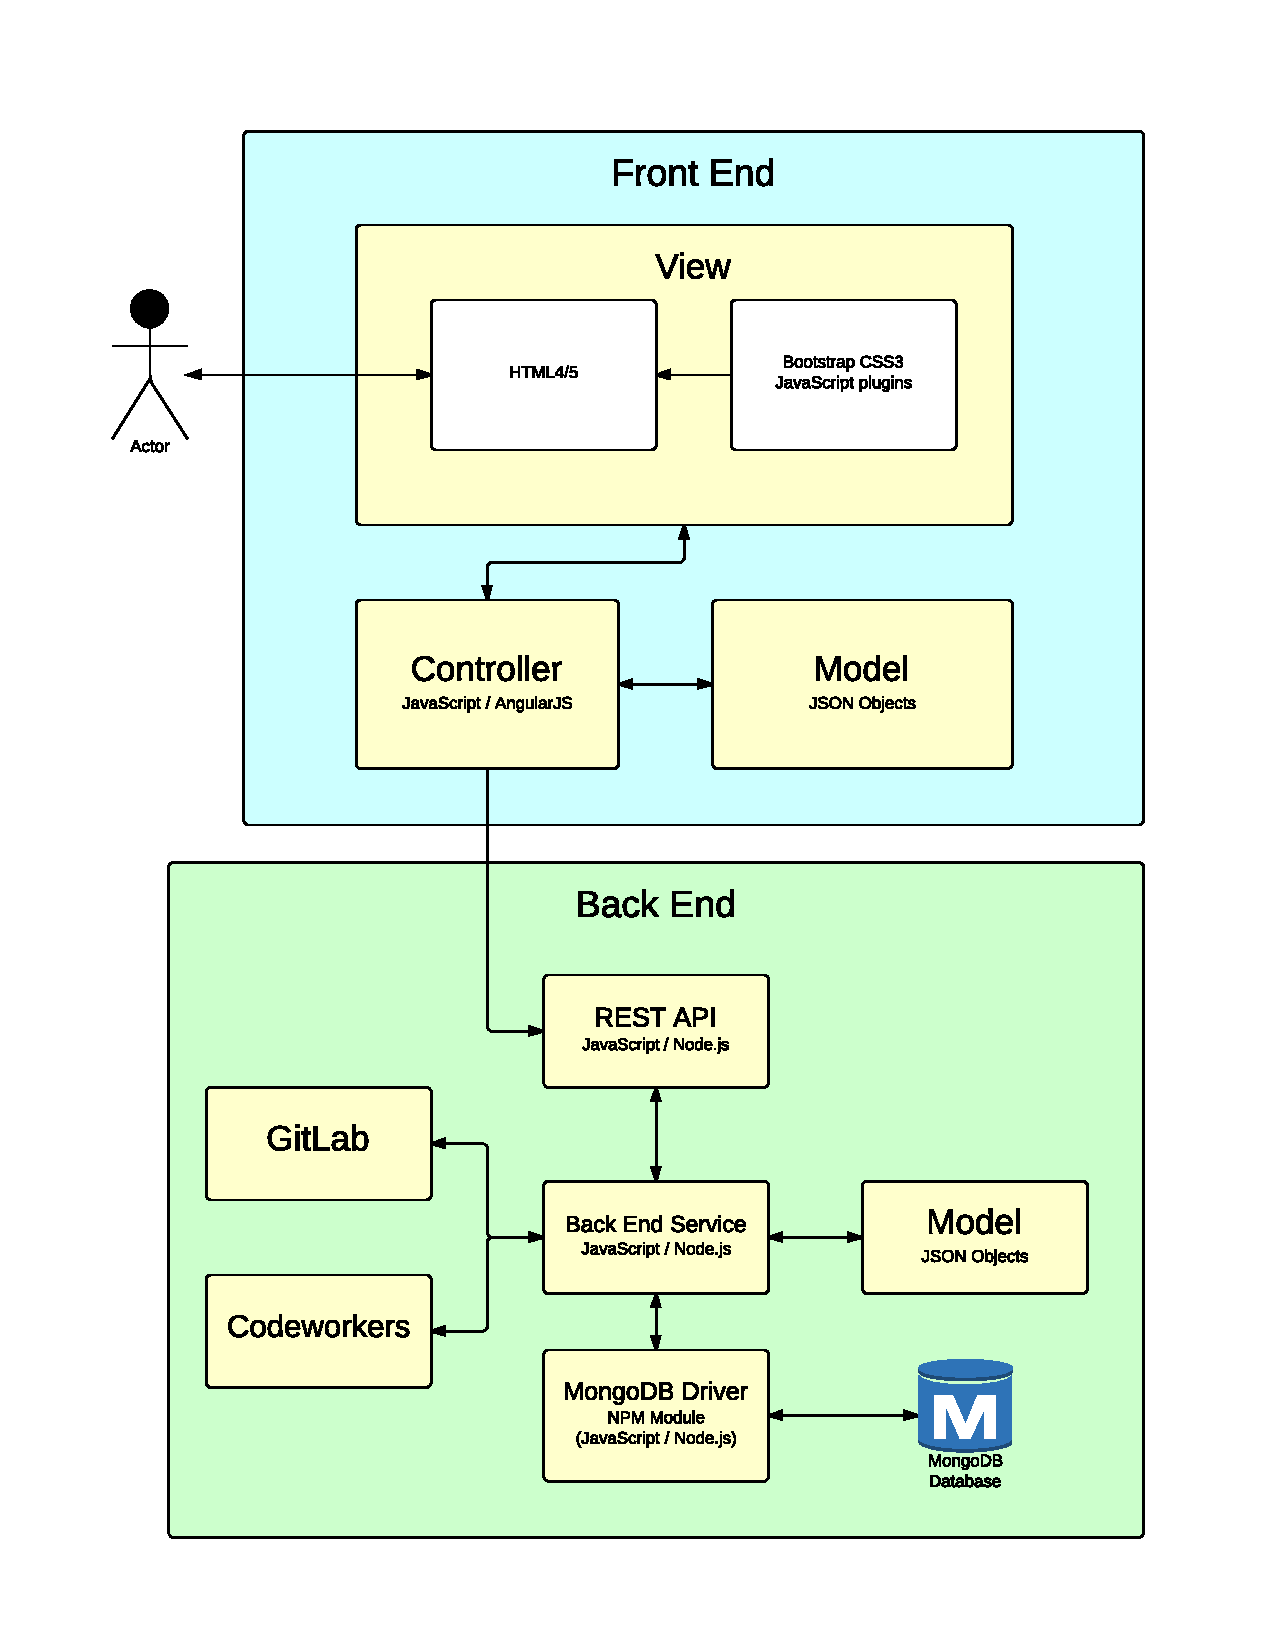
\includepdf[pages={-}]{img/tech_archi.pdf}

%presents and describes design alternatives, and justifies all the choices made

%presents and describes system architecture

%present progress in the design with technical diagrams and description of system components (appendices required for calculations, and detailed documentation diagrams and descriptions)

%analyzes and justifies any departures with respect to original plan

%presents snapshots or other evidences

%check list:

%present system design overview
%present sys conceptual design (how it will look like)
%present software architecture
%present component description
%present user interface
%presents software progress assessment
%presents class diagrams
%presents software design justications
%presents communication interfaces